\chapter{Datasets inspection}
\label{chap:Datasets}

In the context of the conducted research, the selection and analysis of datasets play a fundamental role in understanding and addressing the challenges presented in this task. This chapter delves into the datasets chosen as the foundation for investigations, as these data serve as the raw material from which crucial information is extracted for analysis. By systematically considering the origins, dimensions, and peculiarities of these datasets, we can establish a foundation for comprehending the dynamics that define this field of study.
As mentioned in the previous chapter, one of the main challenges in analyzing pollution data is the presence of erroneous or missing data, often caused by faulty or dirty sensors. 
It is important to consider outliers, as they may represent either actual observations of a significant increase in pollutants or random errors in the sensor. The location of the sensor is also a crucial factor that can affect the average values of the series. 
To account for this variability in the data based on location, three datasets have been selected for analysis, namely:
\begin{itemize}
    \item Citypulse (containing data from Aarhus, Denmark),
    \item Seoul pollution data,
    \item Madrid pollution data.
\end{itemize}

These three cities are located in three different regions, each with its own unique lifestyle, morphology, and climate.

\section{Data availabilty}
\subsection{Citypulse}
Created in the context of the CityPulse EU FP7 Project, this collection of datasets contains a lot of annotated data, relevant in the context of a smart city \cite{CityPulseDataset}. For this analysis, the following datasets have been chosen:
\begin{itemize}
    \item \textbf{Pollution data}
    \item Road traffic data
    \item Weather data
    \item Parking data
\end{itemize}

It is highlighted in the website that while the other three datasets are provided as observations from real sensors, the pollution dataset is generated using a simple function that uses controlled randomness to provide a realistic and bounded measurement\footnote{The stream generation for sensor measurements involves updating values every 5 minutes. If the initial value is below 20, it increases by a random integer between 1 and 10. If the value exceeds 210, it decreases by a random integer between 1 and 10. Otherwise, it changes by a random integer between -5 and 5 to create a realistic and bounded measurement stream.}. To avoid using this generated data, which would likely bias the results of our prediction algorithms, actual values of the available pollutants are extracted from another source \cite{EEA_AirQuality}.
The dataset spans from August 2014 to October 2014 and contains a total of 10,560 observations. Each observation is recorded at regular intervals of 5 minutes. However, for the purpose of this analysis, we resample the data on an hourly basis. 
Missing data in the time series are imputed via linear interpolation, as most of the variables did not have long series of consecutive missing data.

\begin{table}[h]
\centering
\begin{tabular}{|c|c|}
\hline
\textbf{Category} & \textbf{Variables} \\ \hline
Air Pollution Observations & \begin{tabular}[c]{@{}c@{}}O\textsubscript{3}, PM\textsubscript{10}, \\PM\textsubscript{2.5}, NO\textsubscript{2}\end{tabular} \\ \hline
Meteorological Data & \begin{tabular}[c]{@{}c@{}}temp, feelslike, humidity, precip,\\ precipprob, windspeed, cloudcover, visibility\end{tabular} \\ \hline
Traffic and Parking Data & \begin{tabular}[c]{@{}c@{}}vehicleCount, avgSpeed, \\ Totalspaces,occupied, occupancy\end{tabular} \\ \hline
\end{tabular}
\caption{Variables in the CityPulse Dataset. Description of each variable is found on Table \ref{apptable:Citypulse_variable_descriptio} in the appendix.}
\end{table}

\newpage

\begin{figure}[h]
    \centering
    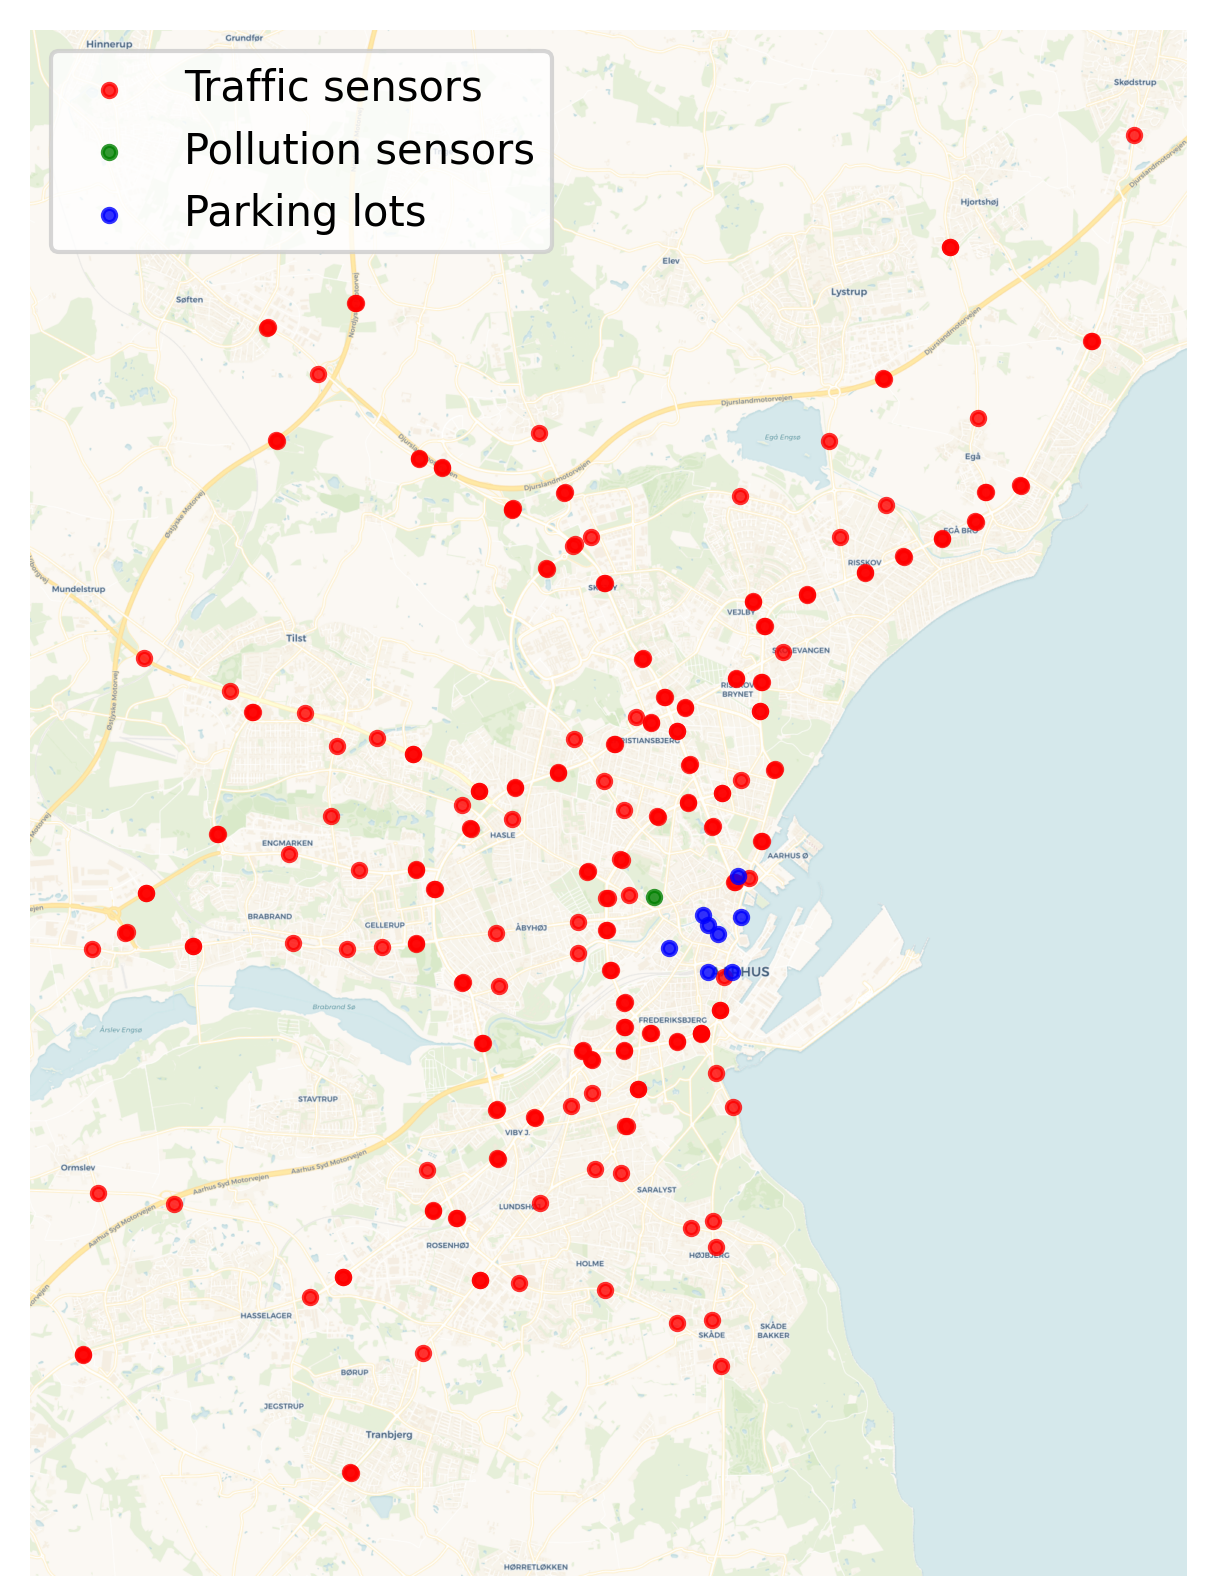
\includegraphics[width=0.5\linewidth]{images/aarhussensors.png}
    \caption{Map of Aarhus city sensors, in red are the traffic sensors, in green the only sensor for pollutants measurements, in blue the parking lots.}
    \label{fig:aarhus-sensors}
\end{figure}


\subsection{Seoul}
As mentioned in chapter \ref{subsec:ExamplesOfSmartCities}, the Seoul Metropolitan Government provides public air pollution data through the Open Data Plaza. However, the data for this activity is collected from Kaggle \cite{kaggleSeoul}, where the data for six pollutants (SO\textsubscript{2}, NO\textsubscript{2}, CO, O\textsubscript{3}, PM\textsubscript{10}, PM\textsubscript{2.5}) is already aggregated into a single table containing hourly observations from January 2017 to December 2019. 
In this dataset, observations from 25 stations located in different districts of Seoul are available. However, to make the results comparable between the three datasets, only one station is used for analysis and model training (Figure \ref{fig:SeoulSensors}).
To supplement the data with additional information, weather data were downloaded from the Open-Meteo website \cite{openMeteo}, which provides an API to download historical data with hourly granularity. 

\begin{table}[h]
\centering
\begin{tabular}{|c|c|}
\hline
\textbf{Category} & \textbf{Variables} \\ \hline
Air Pollution Observations & \begin{tabular}[c]{@{}c@{}}O\textsubscript{3}, PM\textsubscript{10}, PM\textsubscript{2.5},\\ NO\textsubscript{2}, CO, SO\textsubscript{2}\end{tabular} \\ \hline
Meteorological Data & \begin{tabular}[c]{@{}c@{}}temp, humidity, precip,\\ windspeed, cloudcover, rain, snow\end{tabular} \\ \hline
\end{tabular}
\caption{Variables in the Seoul Dataset. Description of each variable is found on Table \ref{apptable:Seoul_variable_description} in the appendix.}
\end{table}


\begin{figure}[h]
    \centering
    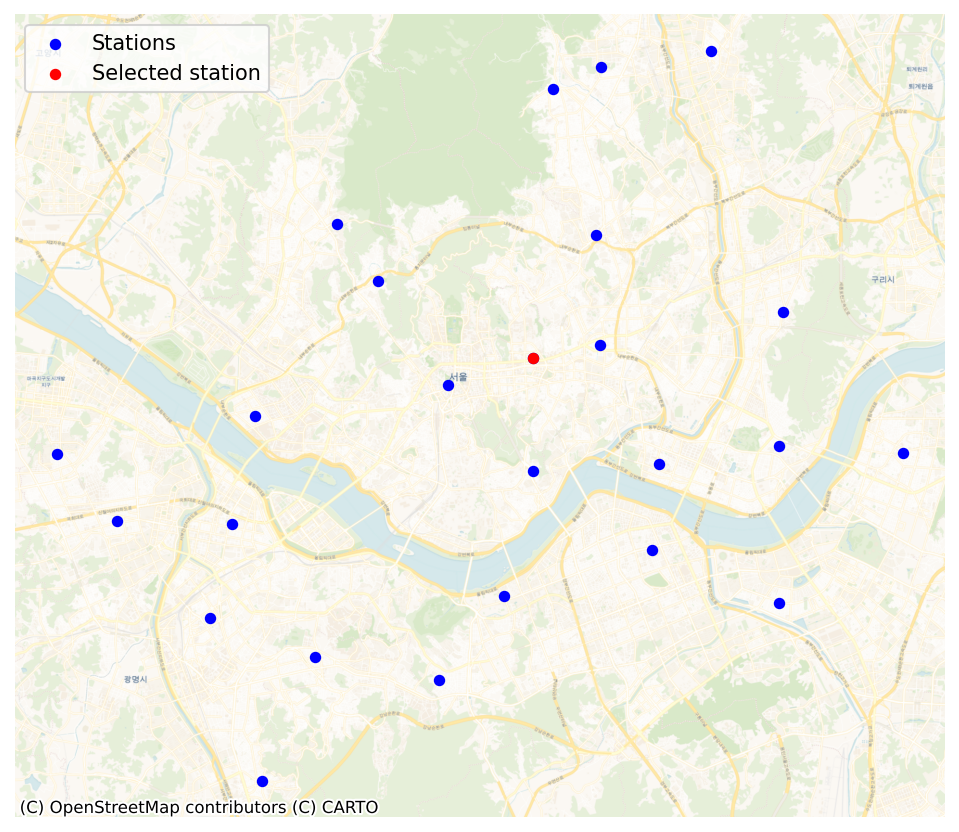
\includegraphics[width=0.5\linewidth]{images/seoulsensors.png}
    \caption{Seoul measurement stations across the districts. In red the station elected for this analysis.}
    \label{fig:SeoulSensors}
\end{figure}

\subsection{Madrid}
The air quality data for Madrid is publicly available on the Madrid's City Council Open Data website \cite{openDataMadrid}. Being data downloadable from the website in a confusing and not common format, and not well designed for general purpose use, a version of the dataset from Kaggle \cite{kaggleMadrid} has been used in this analysis.
In the DataFrame, particle measurements are recorded for each station, covering the period from January 2001 to April 2018, provided that the station was operational throughout this timeframe. It's important to note that stations differ in their equipment, leading to each station being capable of measuring only a specific subset of particles. For the purposes of this work, we have analyzed data from only one station (Figure \ref{fig:madridsensors}) that collects the six pollutants of interest, and the time range was restricted to three years (2015 - 2017). 
Missing data in some observations, were filled with the previous valid observation.
Again, weather data has been gathered from Open-Meteo website to add information to this dataset.

\begin{table}[h]
\centering
\begin{tabular}{|c|c|}
\hline
\textbf{Category} & \textbf{Variables} \\ \hline
Air Pollution Observations & \begin{tabular}[c]{@{}c@{}}PM\textsubscript{10}, PM\textsubscript{2.5}, NO\textsubscript{2}, \\ CO,	SO\textsubscript{2}, O\textsubscript{3}\end{tabular} \\ \hline
Meteorological Data & \begin{tabular}[c]{@{}c@{}}temp, humidity, dew, precip,\\ rain, snow, pressure, windspeed, \\ cloudcover, winddir\end{tabular} \\ \hline
\end{tabular}
\caption{Variables in the Madrid Dataset. Description of each variable is found on Table \ref{apptable:madrid_variable_description} in the appendix.}
\end{table}


\begin{figure}[h]
    \centering
    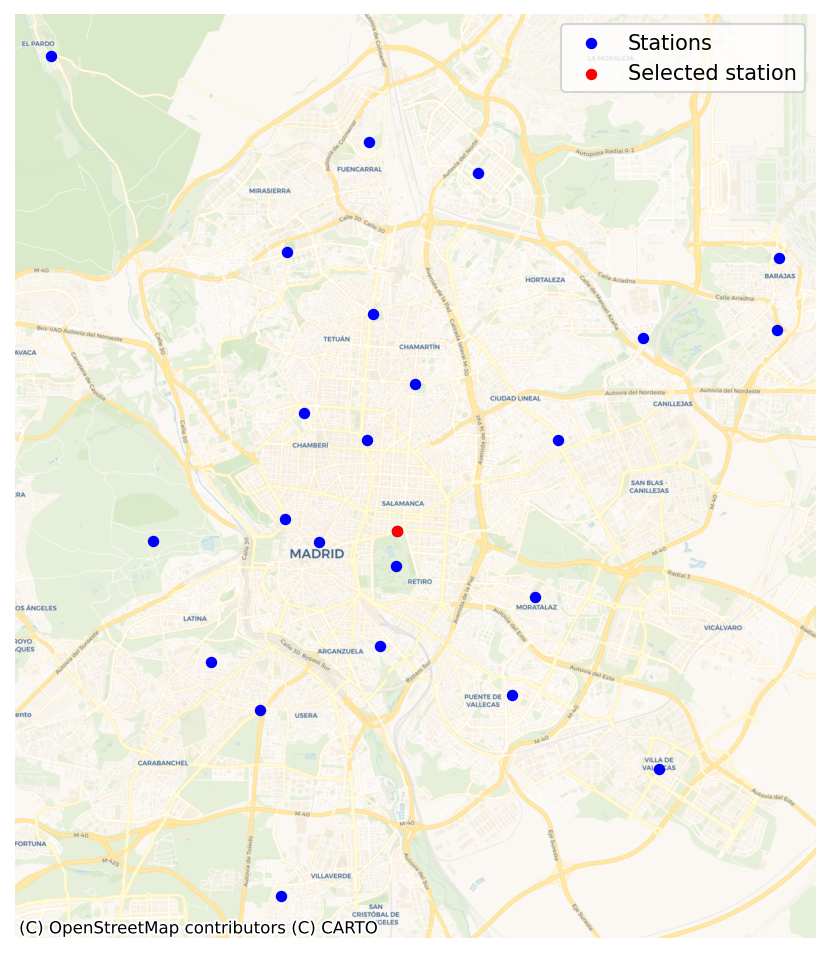
\includegraphics[width=0.5\linewidth]{images/madridsensors.png}
    \caption{Madrid measurement stations. In red the station elected for this analysis.}
    \label{fig:madridsensors}
\end{figure}

\newpage
\section{Explorative data analysis}
In this section is provided a brief data analysis to understand the dataset properties.

\subsection{Citypulse}

The graphical representation (Figure \ref{fig:ts_citypulse}) reveals that the time series of all four pollutants exhibit irregular and variable trends. The Ozone and PM\textsubscript{2.5} variables demonstrate nearly identical, on average decreasing patterns. Conversely, the PM\textsubscript{10} historical series displays a more sporadically linear trend, especially during descents, likely attributed to atmospheric events such as rainfall. The NO\textsubscript{2} historical series follows a less linear trend, frequently approaching zero. Notably, an anomalous trend occurs in the first week of October, which can be attributed to the interpolation method employed for handling missing data.

\begin{figure}[h]
    \centering
    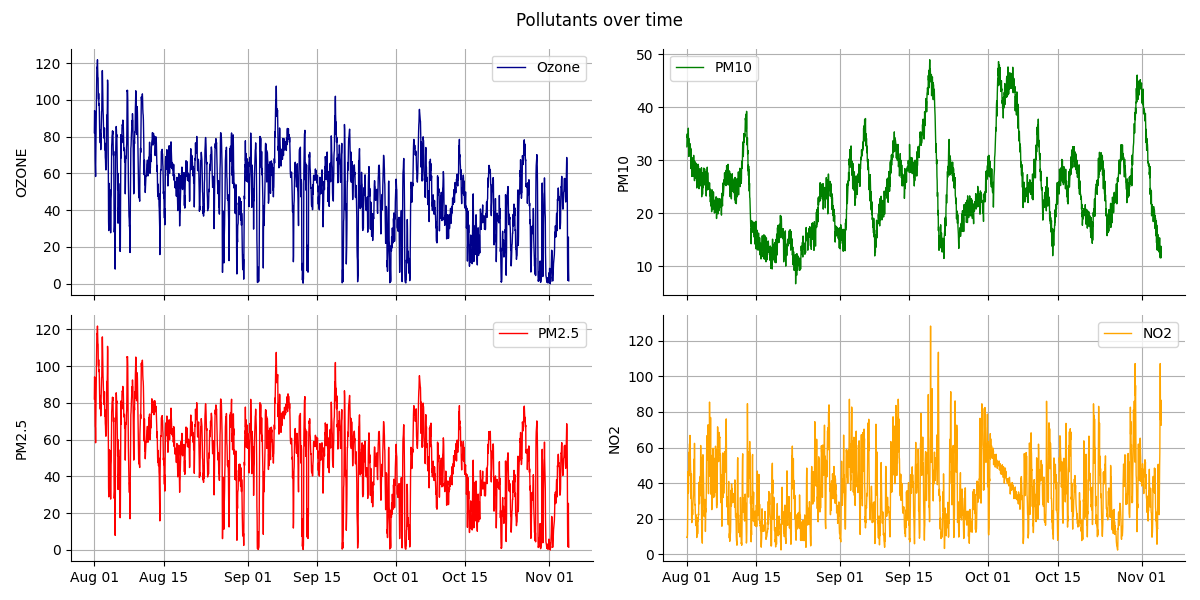
\includegraphics[width=1\linewidth]{images/ts_citypulse.png}
    \caption{Pollutant concentrations over time for the Citypulse dataset}
    \label{fig:ts_citypulse}
\end{figure}

Let us now examine the correlation among all variables in the dataset (Figure \ref{fig:corr_matrix_citypulse}):
\begin{itemize}

    \item The variables "occupied" and "occupancy" are naturally correlated, as one is computed based on the other.
    \item "temp" and "feelslike" exhibit a strong positive correlation, nearly perfect at 0.995244, as expected since they represent similar measurements of meteorological conditions.
    \item The two target variables, ozone and PM\textsubscript{2.5}, are perfectly correlated, and this should be taken into consideration in model construction.
    \item Ozone and PM\textsubscript{2.5} variables show positive correlations with the "temp" and "feelslike" variables, suggesting a potential association between these variables.
    \item Unexpectedly, the PM\textsubscript{10} and PM\textsubscript{2.5} variables do not show a strong correlation, as would be expected and we will see instead in the other two datasets.
\end{itemize}

\begin{figure}[h]
    \centering
    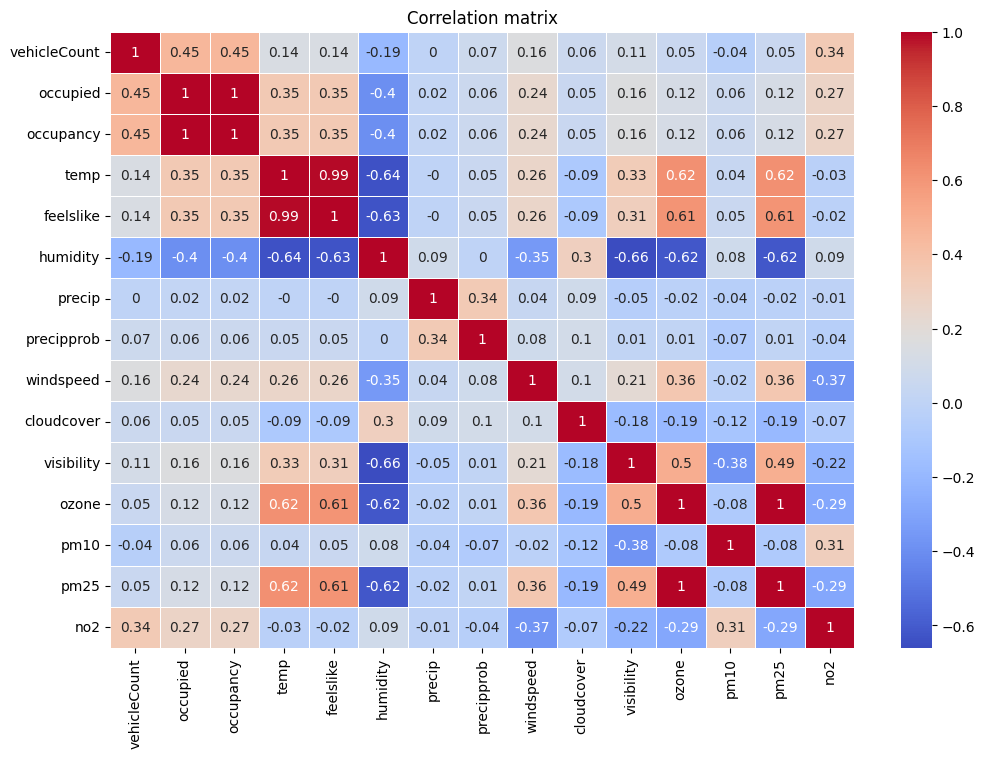
\includegraphics[width=0.75\linewidth]{images/corr_matrix_citypulse.png}
    \caption{Correlation matrix between the variables of the Citypulse dataset.}
    \label{fig:corr_matrix_citypulse}
\end{figure}

\newpage
\subsection{Seoul}

Analyzing the time series of pollutants in Seoul (Figure \ref{fig:ts_seoul}) reveals several distinct patterns. In the cases of SO\textsubscript{2} and CO, peaks coincide on specific dates. Notably, CO levels constitute approximately 10\% of SO\textsubscript{2} levels. However, peak durations are limited to 2-3 observations, followed by an abrupt decline, raising concerns about observation accuracy. 
A similar pattern emerges in PM\textsubscript{10} and PM\textsubscript{2.5}, underscoring the correlation between these two series. The historical O\textsubscript{3} series exhibits elevated levels during warmer months, contrasting with lower levels during colder months.
Conversely, NO\textsubscript{2} displays an opposing trend, with reduced variability in warmer months and elevated levels in colder months. 

\begin{figure}[h]
    \centering
    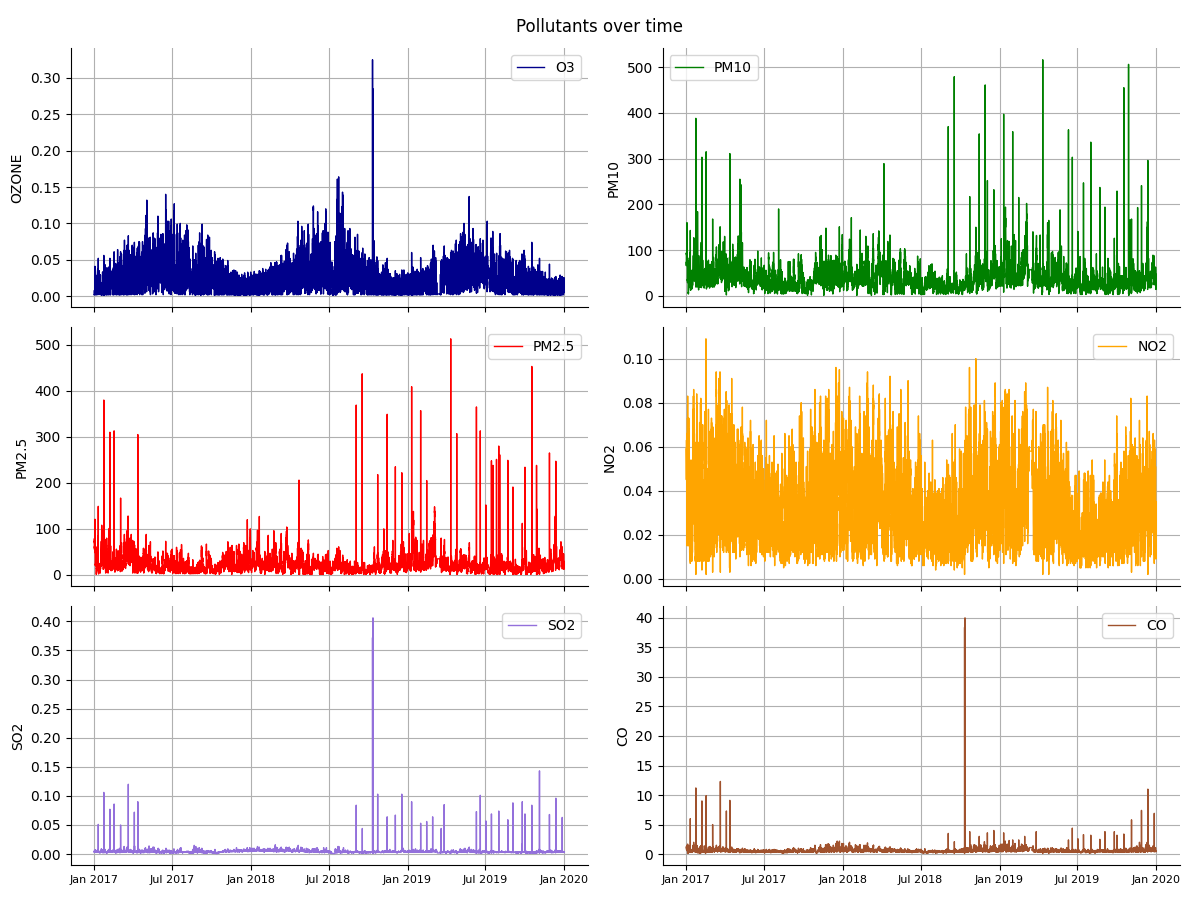
\includegraphics[width=1\linewidth]{images/ts_seoul.png}
    \caption{Pollutant concentrations over time for the Seoul dataset}
    \label{fig:ts_seoul}
\end{figure}


As observed in the plots, substantial correlations are evident in the correlation matrix (Figure \ref{fig:corr_matrix_seoul}):

\begin{itemize}
    \item CO and SO\textsubscript{2} exhibit a strong positive correlation (0.79).
    \item PM\textsubscript{2.5} and PM\textsubscript{10} display a notable positive correlation (0.8).
    \item A significant positive correlation is noted between PM\textsubscript{2.5} and CO (0.65).
\end{itemize}
Further insights include a negative correlation between NO\textsubscript{2} and O\textsubscript{3} (-0.55), signifying an inverse relationship. Additionally, we can see the lack of correlation between wind speed and PM\textsubscript{2.5} (-0.031) and PM\textsubscript{10} (0.036) is affirmed, indicating no significant linear relationship, contrary to what might be expected.

\begin{figure}[h]
    \centering
    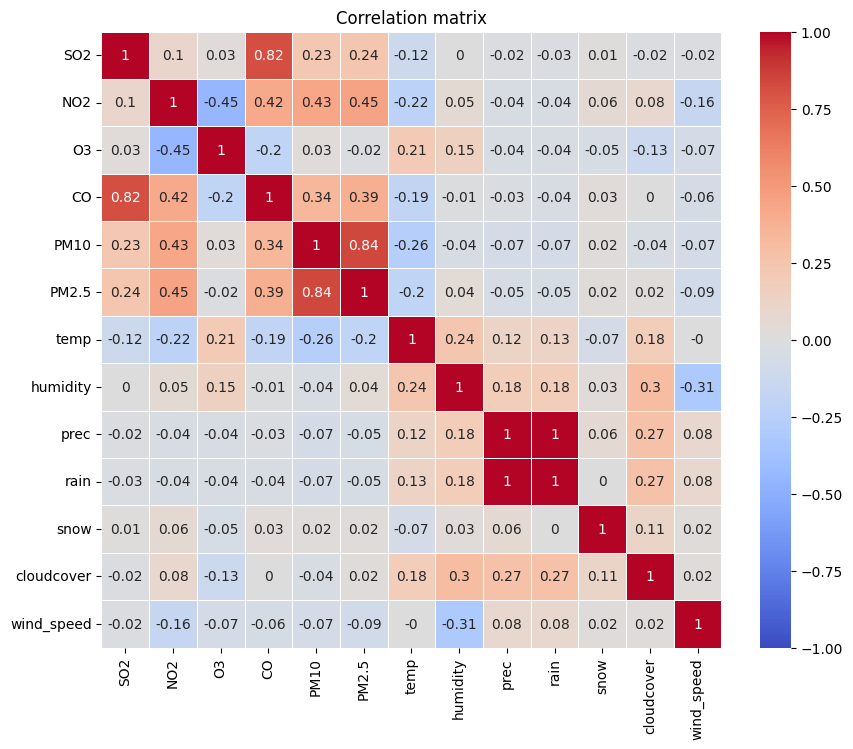
\includegraphics[width=0.75\linewidth]{images/corr_matrix_seoul.png}
    \caption{Correlation matrix between the variables of the Seoul dataset.}
    \label{fig:corr_matrix_seoul}
\end{figure}

\newpage
\subsection{Madrid}
\label{subsec:madrid-eda}
Examining the plots (Figure \ref{fig:ts_madrid}) yields insightful observations:
the behavior of PM\textsubscript{10} and PM\textsubscript{2.5} demonstrates a striking similarity, implying a close connection between these particulate matter metrics.
SO\textsubscript{2} presents an anomalous linear growth in 2017 from April to November, followed by a subsequent return to lower levels. This peculiar pattern suggests a potential sensor replacement, likely occurring in both November 2017 and July 2016.
Nitric dioxide (NO) exhibits high variability, indicative of dynamic fluctuations, yet maintains an overall stable trend, highlighting consistent concentrations of this pollutant.
In alignment with the historical Seoul data, O\textsubscript{3} concentrations follow a seasonal dynamic, increasing during warmer months and decreasing in winter. This cyclical pattern reflects the climatic influence on ozone levels.

\begin{figure}[h]
    \centering
    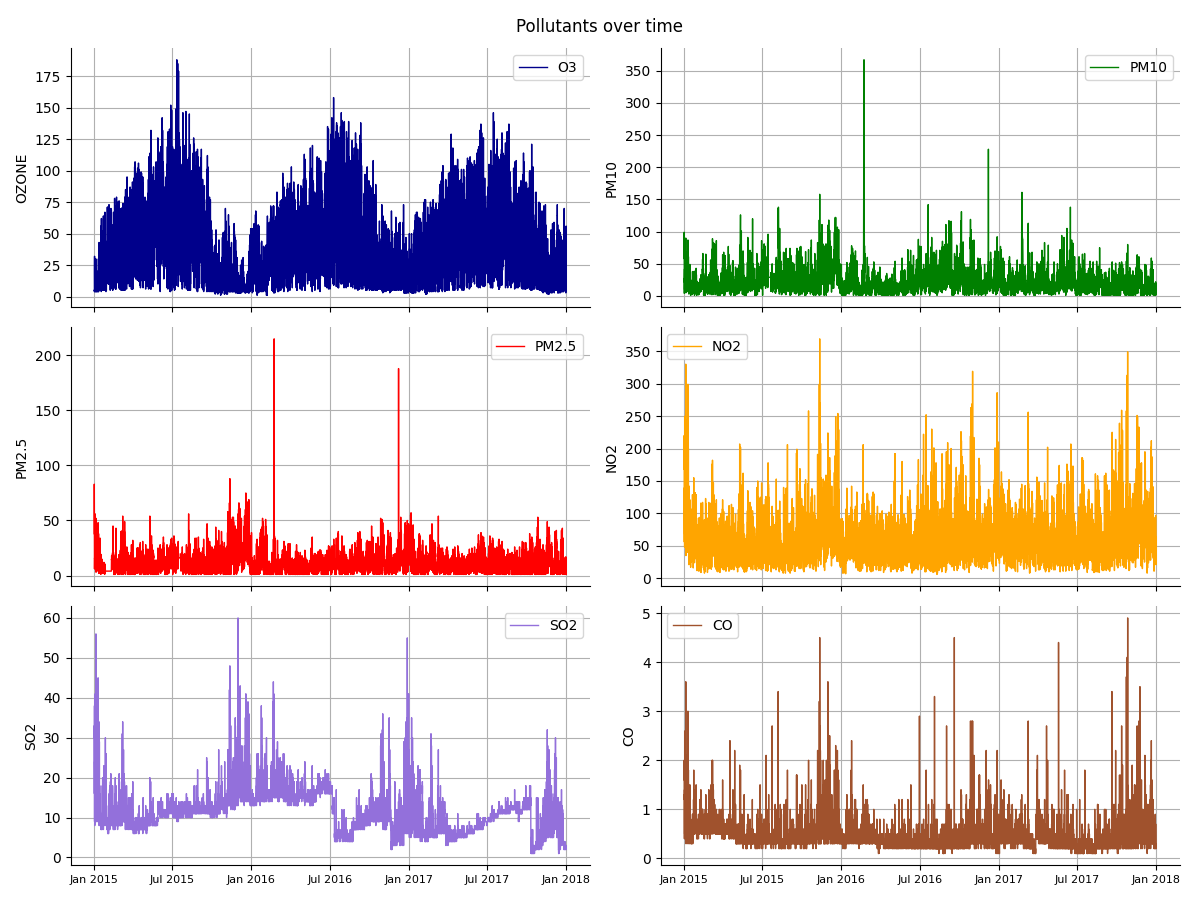
\includegraphics[width=1\linewidth]{images/ts_madrid.png}
    \caption{Pollutant concentrations over time for the Madrid dataset}
    \label{fig:ts_madrid}
\end{figure}

The correlation matrix (Figure \ref{fig:corr_matrix_madrid}) analysis reveals noteworthy connections: 
\begin{itemize}
    \item  A strong positive correlation (0.72) indicates a significant association between carbon monoxide (CO) and nitrogen dioxide (NO\textsubscript{2}), suggesting shared emission sources or interdependence in atmospheric processes.
    \item A high positive correlation (0.85) between PM\textsubscript{2.5} and PM\textsubscript{10} again suggests a robust coherence in the dynamics of fine and coarse particulate matter, indicative of shared sources or mutual influences.
    \item A notable negative correlation (-0.56) between nitrogen dioxide (NO\textsubscript{2}) and ozone (O\textsubscript{3}) suggests an antagonistic interaction, potentially influenced by disparate sources or chemical reactions in the atmosphere. This pattern is consistent with findings in the Seoul dataset.
\end{itemize}

\begin{figure}[h]
    \centering
    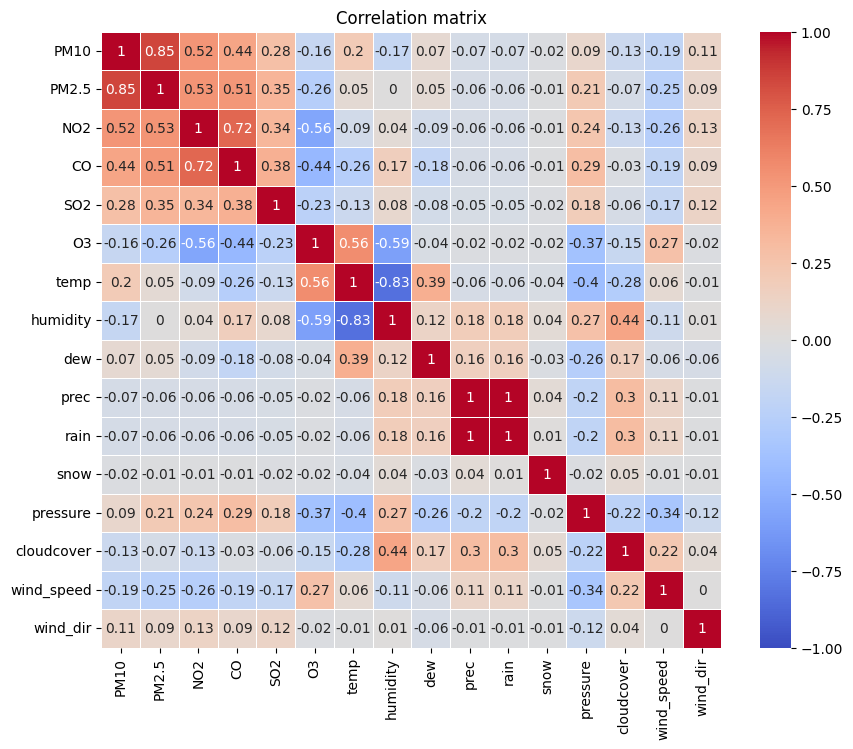
\includegraphics[width=0.75\linewidth]{images/corr_matrix_madrid.png}
    \caption{Correlation matrix between the variables of the Madrid dataset.}
    \label{fig:corr_matrix_madrid}
\end{figure}

\newpage
\section{In-depth analysis}

The subsequent phase of the dataset analysis will be dedicated exclusively to time series analysis. However, before delving into this analysis, it is useful to introduce three fundamental concepts that will enhance comprehension of the forthcoming examination.

\paragraph{Seasonal decomposition:}Seasonal decomposition is a statistical technique employed to dissect time series data into fundamental components, namely trend, seasonality, and residual. The trend signifies long-term alterations, elucidating the overall trajectory of the data; seasonality captures cyclic patterns within predefined time intervals; and residual accounts for the stochastic variation that remains subsequent to the consideration of both trend and seasonality.
This method serves diverse purposes, such as \textbf{pattern identification}, removal of seasonal effects, enhancement of predictive capabilities, and facilitation of \textbf{comparative analysis}. Notably, the technique can manifest as either additive, wherein components are amalgamated through addition, or multiplicative, where the components are combined through multiplication. The selection of the appropriate method hinges upon the nature of the time series under examination.

\paragraph{Autocorrelation Function (ACF) and Autocorrelation Plot:}The Autocorrelation Function (ACF) is a statistical measure assessing the correlation between a given data point and its preceding points within the same time series. It aids in identifying trends or relevant periodic patterns in past observations. In an ACF plot, values above the dashed line signify positive correlations, while those below indicate negative correlations. Significant peaks outside the confidence interval denote time lags with strong correlations, suggesting potential patterns or seasonality in the time series.

\paragraph{Partial Autocorrelation Function (PACF) and Partial Autocorrelation Plot:}The Partial Autocorrelation Function (PACF) is a measure evaluating the correlation between a given data point and its previous points, accounting for the influence of intervening lags. It proves useful in identifying the direct correlation between a data point and past points without the influence of intermediate lags. In the PACF plot, peaks outside the confidence interval represent time lags with significant correlations not explained by intervening lags. These peaks assist in directly pinpointing relationships between data points, highlighting the most immediate and relevant correlations in the time series. However, interpreting the PACF plot can be difficult by definition.

% TODO - Qua non saprei se includere i plot della PACF oppure no, perchè comunque non ne estraiamo informazioni, sarebbe più un discorso di completezza che di utilità
Usually, ACF and PACF plots are useful to determine the best parameters for the definition of an ARIMA model. However, this is not the case, as these are used only to understand what is the relationship between observations at different times, and the focus will be only on the ACF plot, as it's interpretation in more intuitive and useful for this analysis.

\subsection{Citypulse}
Decomposition of the Aarhus pollutants time series has been carried out using an additive method, setting a period of 168 (24 observations per day * 7 days per week) to accentuate weekly seasonality. Figure \ref{fig:seasonality_aarhus} showcases the results, providing valuable insights into the observed patterns:

\begin{figure}[h]
    \centering
    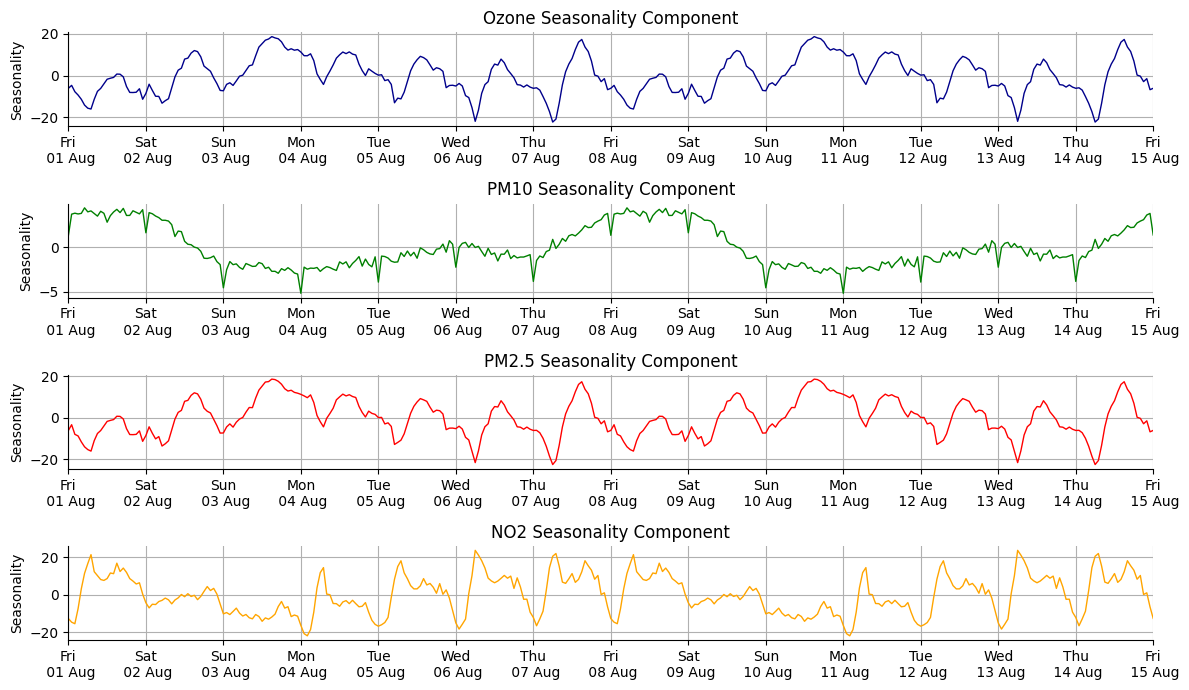
\includegraphics[width=1\linewidth]{images/citypulse_seasonality.png}
    \caption{Seasonal components of Aarhus's pollutants, focusing on a two-week period.}
    \label{fig:seasonality_aarhus}
\end{figure}

\begin{itemize}
\item The seasonal components of Ozone and PM\textsubscript{2.5} exhibit identical patterns. These patterns manifest in two discernible trends: firstly, a reduction in pollutant levels during nighttime hours, followed by an increase during daytime. Secondly, during weekends, the average values of the series demonstrate a tendency to be lower.
\item The seasonal component of PM\textsubscript{10} displays a comparable pattern, wherein it experiences a decline from Saturday to Monday, followed by an increase during weekdays, reaching its zenith on Fridays and Saturdays. However, a unique behavior is observed in PM\textsubscript{10} that is absent in other series, characterized by a precipitous decline in observations at midnight, succeeded by a marked increase in subsequent observations.
\item NO\textsubscript{2} demonstrates a behavior akin to that of Ozone and PM\textsubscript{2.5}, with higher values observed during weekdays and lower values from Saturday to Monday.
\end{itemize}

Moving forward, present plots illustrating the autocorrelation function are presented. With respect to the ACF and a scrutiny of the plots (depicted in Figure \ref{fig:acfplot_citypulse}), several considerations can be derived:

\begin{figure}[h]
    \centering
    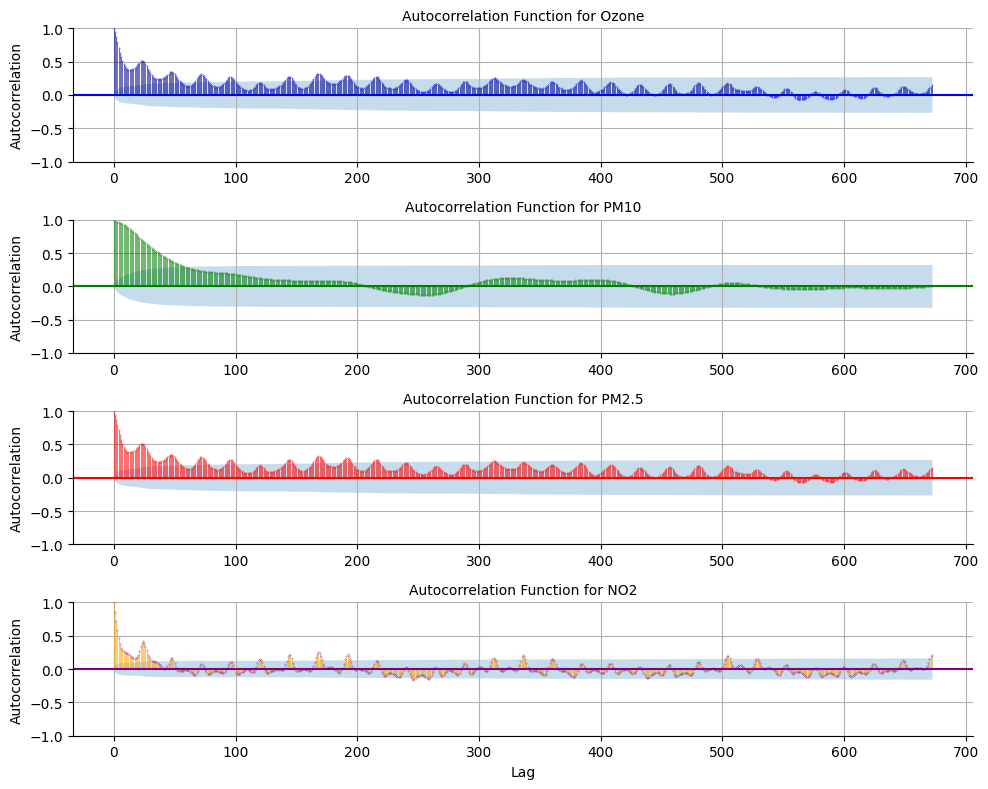
\includegraphics[width=1\linewidth]{images/acfplot_citypulse.png}
    \caption{ACF Plot for pollutants in Aarhus, displaying the first 700 values of the autocorrelation function.}
    \label{fig:acfplot_citypulse}
\end{figure}

\begin{itemize}
    \item \textbf{O\textsubscript{3}:}
    The autocorrelation function computed on the ozone time series (similar to that of PM\textsubscript{2.5}) reveals spikes every 24 lags, indicating a daily seasonality. Additionally, a subtle increase is observed every 168 lags, suggesting a weekly seasonality.
    \item \textbf{PM\textsubscript{10}:}
    Contrary to ozone and PM\textsubscript{2.5}, the autocorrelation function for the PM\textsubscript{10} time series does not exhibit distinct patterns. Observations seem to be simply correlated with the approximately preceding 50 observations.
    \item \textbf{NO\textsubscript{2}:}
    Autocorrelation analysis of the NO\textsubscript{2} time series demonstrates a pronounced spike every 24 lags, corresponding to a daily seasonality. Furthermore, there is a growth trend every 168 lags, indicating a weekly seasonality. This suggests that observations are correlated not only within a day or two but also over the span of one or two weeks.

\end{itemize}






\subsection{Seoul}
Seoul pollutants time series have been decomposed using additive method, specifying a period of 168 (24 observations per day * 7 days per week), in order to highlight seasonality between weeks.
From this analysis (Figure \ref{fig:seasonality_seoul}) we can note several things:

\begin{figure}[h]
    \centering
    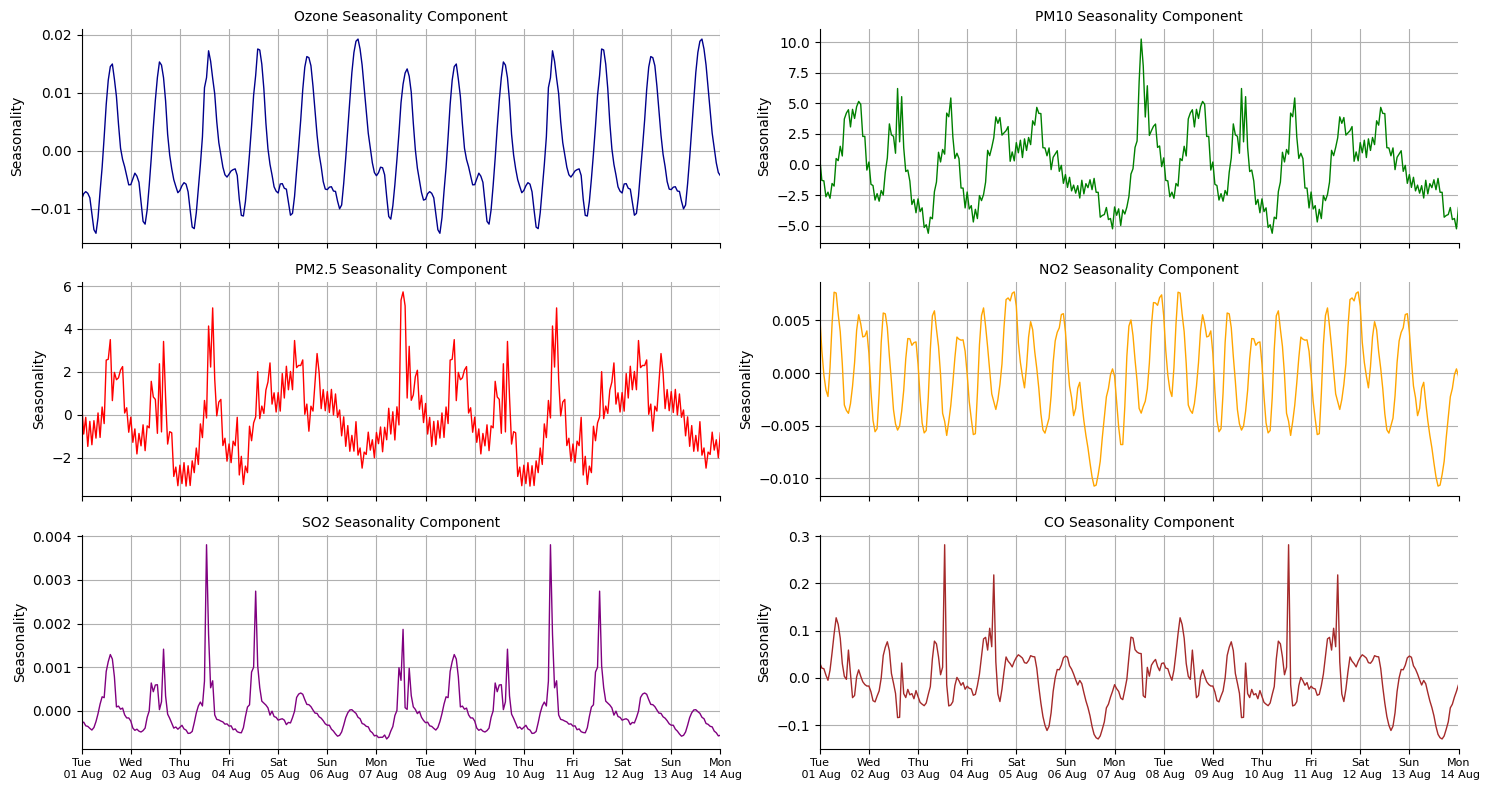
\includegraphics[width=1\linewidth]{images/seoul_seasonality.png}
    \caption{Seasonal components of Seoul's pollutants, focusing on a two-week period.}
    \label{fig:seasonality_seoul}
\end{figure}

\begin{itemize}
    \item \textbf{O\textsubscript{3}} shows peaks during the day, approximately around noon, and rapidly decreases towards the evening, reaching the minimum. Lower values are observed on Saturdays, Mondays, and Tuesdays.
    \item \textbf{PM\textsubscript{10}} decreases on Saturday, Sunday, and Monday, then increases during the week.
    \item \textbf{PM\textsubscript{2.5}}, in contrast to PM\textsubscript{10}, does not exhibit specific patterns, other than the usual increase during the day and decrease during the night.
    \item \textbf{NO\textsubscript{2}} shows two peaks per day, with the most significant peaks occurring on Saturdays, and negative peaks on Sundays.
    \item \textbf{SO\textsubscript{2}} exhibits peaks on weekdays and remains low during the weekend.
    \item \textbf{CO} demonstrates a general increase throughout the week and a decrease over the weekend until Monday, where the lowest values are recorded.
\end{itemize}

Next, plots for the autocorrelation function are displayed. As for the ACF, looking at the plots (Figure \ref{fig:acfplot_seoul}), the following considerations can be made:

\begin{figure}[h]
    \centering
    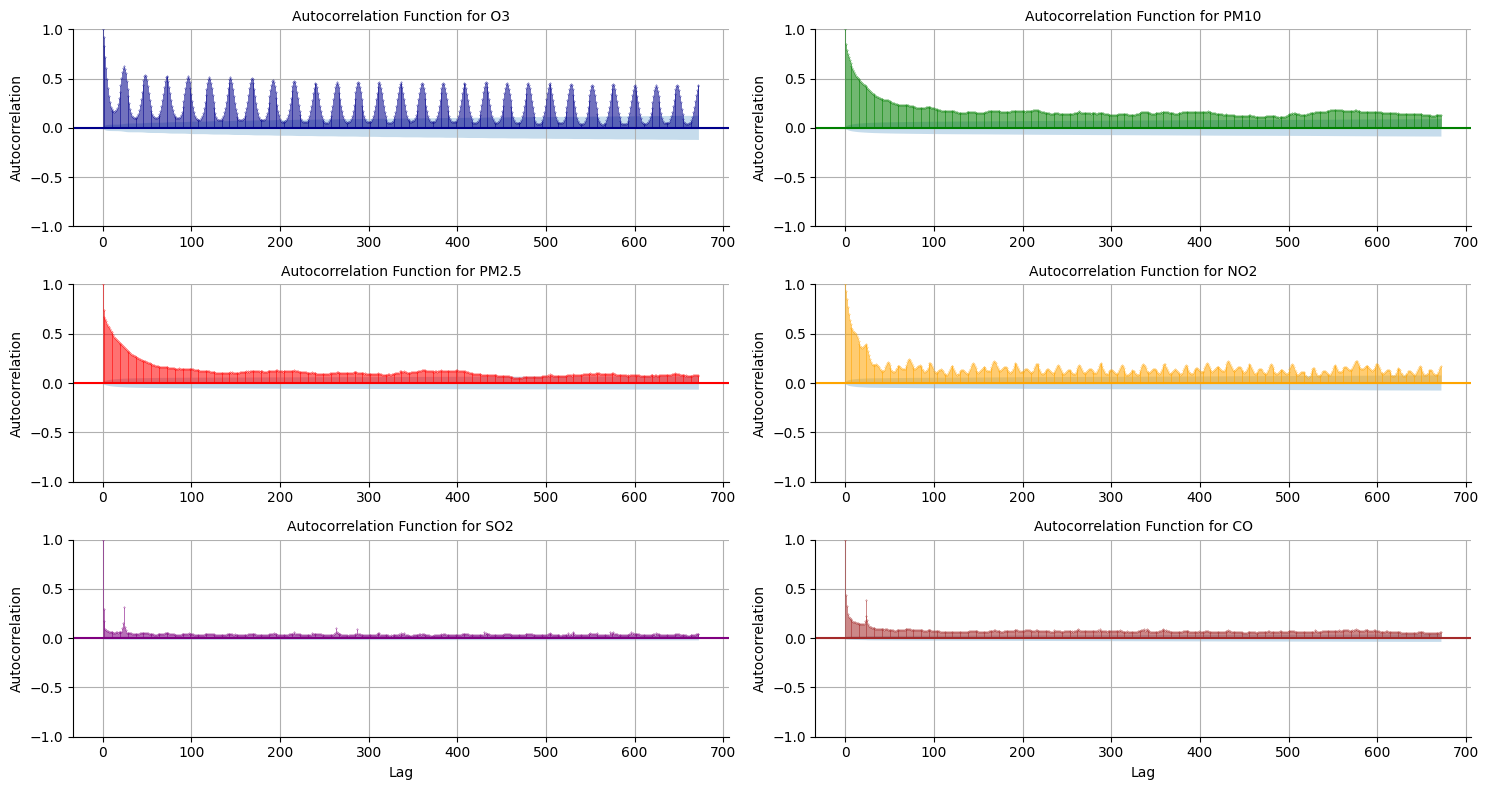
\includegraphics[width=1\linewidth]{images/acfplot_seoul.png}
    \caption{ACF Plot for pollutants in Seoul, displaying the first 700 values of the autocorrelation function.}
    \label{fig:acfplot_seoul}
\end{figure}

\begin{itemize}
    \item \textbf{O\textsubscript{3}} exhibits clear daily seasonality, and there is also a subtle weekly seasonality discernible in the data.
    \item \textbf{PM\textsubscript{10} and PM\textsubscript{2.5}} demonstrate a robust autocorrelation in the initial approximately 60 observations, with a noticeable tendency towards weekly seasonality. However, daily seasonality is not prominently evident.
    \item \textbf{NO\textsubscript{2}} shows peaks approximately every 10 days, along with a strong autocorrelation in the first 24 observations.
    \item \textbf{SO\textsubscript{2}} exhibits daily peaks and some isolated, peculiar spikes that are challenging to explain.
    \item \textbf{CO:} does not display distinct peaks but shows a strong autocorrelation in the initial 24 observations.
\end{itemize}

\subsection{Madrid}
The time series of pollutants in Madrid underwent additive decomposition with a specified period of 168 (24 observations per day multiplied by 7 days per week). Seasonal components resulting from this process are displayed in Figure \ref{fig:madrid_seasonality}:

\begin{figure}[h]
    \centering
    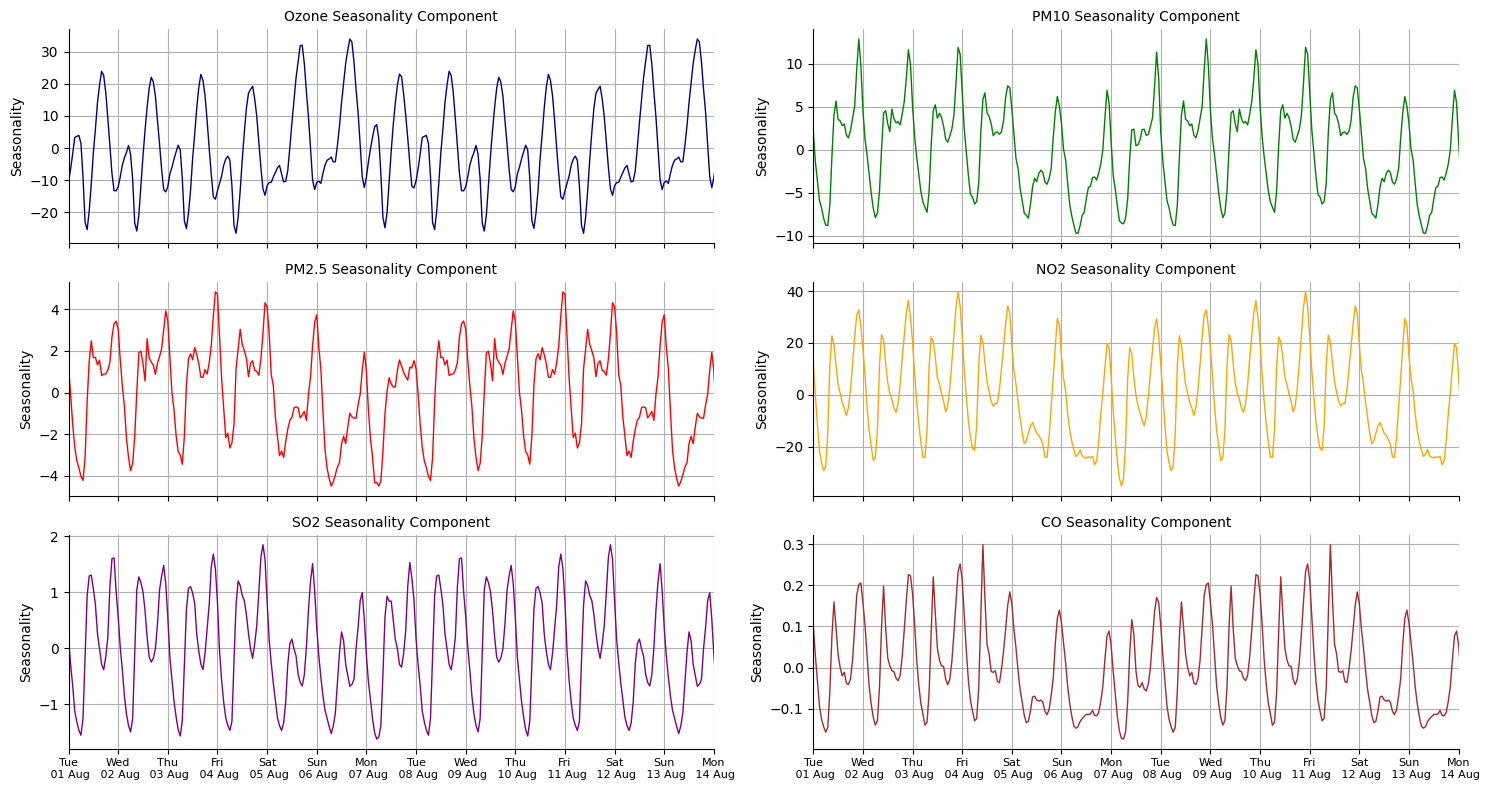
\includegraphics[width=1\linewidth]{images/madrid_seasonality.png}
    \caption{Seasonal components of Seoul's pollutants, focusing on a two-week period.}
    \label{fig:madrid_seasonality}
\end{figure}

\begin{itemize}
    \item \textbf{O\textsubscript{3}} peaks during the day (around noon) and rapidly decreases towards the evening, reaching the minimum. Unlike other pollutants, the highest peaks are observed on weekends.
    \item \textbf{PM\textsubscript{10}} decreases on Friday, Saturday, and Sunday, and increases during the week.
    \item \textbf{PM\textsubscript{2.5}}, in contrast to the historical series in Seoul, follows the same pattern as PM\textsubscript{10}.
    \item \textbf{NO\textsubscript{2}} displays two peaks per day, with the most significant peaks occurring on Saturdays, and negative peaks on Sundays.
    \item \textbf{SO\textsubscript{2}} exhibits a seasonal component with higher variance on weekdays and lower variance on weekends.
    \item \textbf{CO} demonstrates a general increase throughout the week and a decrease over the weekend until Monday, where the lowest values are recorded.
\end{itemize}

Following this, the autocorrelation function plots are presented. Analyzing the ACF plots (Figure \ref{fig:acfplot_madrid}), the subsequent observations can be noted:

\begin{figure}[h]
    \centering
    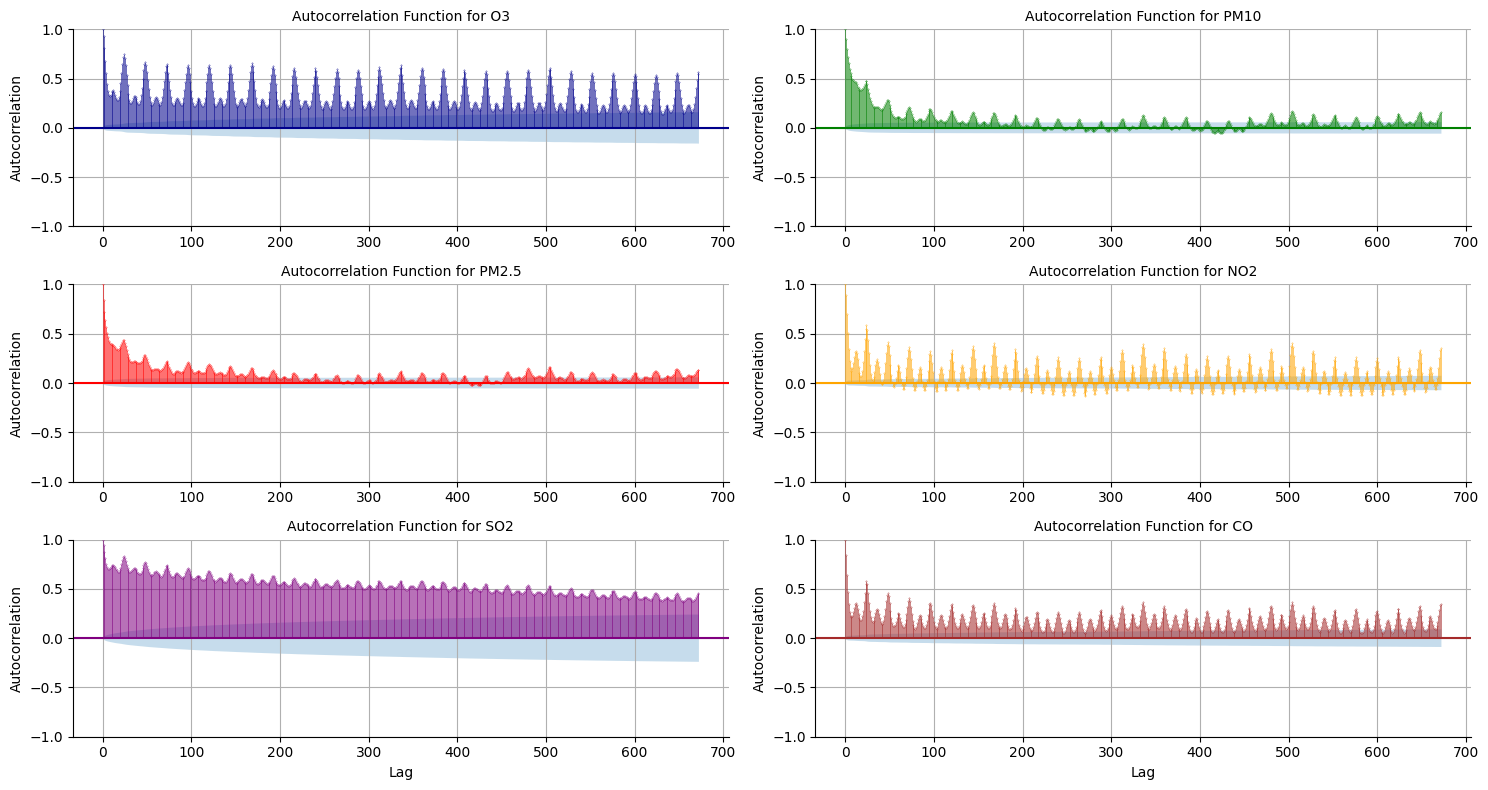
\includegraphics[width=1\linewidth]{images/acfplot_madrid.png}
    \caption{ACF Plot for pollutants in Madrid, displaying the first 700 values of the autocorrelation function.}
    \label{fig:acfplot_madrid}
\end{figure}

\begin{itemize}
    \item \textbf{Ozone (O\textsubscript{3})} exhibits a conspicuous daily and intra-daily seasonality. Additionally, a subtle weekly seasonality is observable.
    \item \textbf{Particulate Matter (PM\textsubscript{10} and PM\textsubscript{2.5})} demonstrates a robust autocorrelation in the initial approximately 60 observations. Notably, there is an inclination towards bi-weekly seasonality, coupled with a distinct daily seasonality.
    \item \textbf{Nitrogen Dioxide (NO\textsubscript{2})} shows approximately every 7 days, together with a strong daily and intra-daily autocorrelation.
    \item \textbf{Sulfur Dioxide (SO\textsubscript{2})} features daily peaks and a pronounced initial autocorrelation that diminishes after numerous observations, likely influenced by the peculiar curve pattern.
    \item \textbf{Carbon Monoxide (CO)} displays a daily and intra-daily autocorrelation, alongside a subtle tendency towards weekly seasonality.
\end{itemize}

\newpage
\section{Conclusions}
In this chapter, an examination of the primary facets of the three datasets has been conducted, with a particular emphasis on the time series of pollutants. In order to consolidate the most significant characteristics of the datasets, the following summary table is presented.



\begin{table}[!ht]
    \centering
    
    \begin{tabular}{|l|l|c@{\hspace{4pt}}c@{\hspace{4pt}}c@{\hspace{4pt}}c@{\hspace{4pt}}c@{\hspace{4pt}}c|ccc|}
    \hline
        \multirow{2}{*}{Dataset} & \multirow{2}{*}{Duration} & \multicolumn{6}{c|}{Available pollutants} & \multicolumn{3}{c|}{External features} \\ \cline{3-11}
        & & O\textsubscript{3} & PM\textsubscript{10} & PM\textsubscript{2.5} & NO\textsubscript{2} & SO\textsubscript{2} & CO & Traffic & Parkings & Weather \\ \hline
        \multirow{2}{*}{Citypulse} & 3 Months & \multirow{2}{*}{\checkmark} & \multirow{2}{*}{\checkmark} & \multirow{2}{*}{\checkmark} & \multirow{2}{*}{\checkmark} & & & \multirow{2}{*}{1} & \multirow{2}{*}{1} & \multirow{2}{*}{7} \\ 
        
        & Aug - Nov 2014 &&&&&&&&&\\
        \hline

        
        \multirow{2}{*}{Seoul} & 3 Years & \multirow{2}{*}{\checkmark} & \multirow{2}{*}{\checkmark} & \multirow{2}{*}{\checkmark} & \multirow{2}{*}{\checkmark} & \multirow{2}{*}{\checkmark}& \multirow{2}{*}{\checkmark} & \multirow{2}{*}{0} & \multirow{2}{*}{0} & \multirow{2}{*}{7} \\ 
        
        & 2017 - 2019 &&&&&&&&&\\
        
        \hline


        \multirow{2}{*}{Madrid} & 3 Years & \multirow{2}{*}{\checkmark} & \multirow{2}{*}{\checkmark} & \multirow{2}{*}{\checkmark} & \multirow{2}{*}{\checkmark} & \multirow{2}{*}{\checkmark}& \multirow{2}{*}{\checkmark} & \multirow{2}{*}{0} & \multirow{2}{*}{0} & \multirow{2}{*}{10} \\ 
        
        & 2015 - 2017 &&&&&&&&&\\

        \hline
    \end{tabular}
    \caption{Summary table of the Datasets}
    
\end{table}


The intricacies revealed through these analyses, despite their inherent complexity, prove to be invaluable for comprehending the inherent properties of the respective time series. The identification of distinctive patterns provides essential insights into the temporal dynamics of the environmental variables under consideration.

These findings constitute a crucial foundation for the subsequent stages of model development, where informed decisions must be made regarding the selection of appropriate architectures and parameter configurations. By leveraging the discerned temporal patterns, we can strategically tailor the model definition and data preparation steps to capture and exploit the underlying structures within the time series data.

